%%% Global variables
\newcommand{\weekNum}{1}

\documentclass[12pt]{article}
\usepackage[english]{babel}
\usepackage{natbib}
\usepackage{url}
\usepackage[utf8x]{inputenc}
\usepackage{amsmath}
\usepackage{graphicx}

\graphicspath{{images/}}
\usepackage{parskip}
\usepackage{fancyhdr}
\usepackage{vmargin}
\usepackage{tikz}
\usepackage{pgfgantt}
\usepackage{lscape}
\usetikzlibrary{arrows,shapes,positioning,shadows,trees}
\tikzset{
  basic/.style  = {draw, text width=4cm, drop shadow, font=\sffamily, rectangle},
  root/.style   = {basic, rounded corners=2pt, thin, align=center,
                   fill=blue!20},
  level 2/.style = {basic, rounded corners=6pt, thin,align=center, fill=blue!10,
                   text width=8em},
  level 3/.style = {basic, thin, align=left, fill=pink!30, text width=6.5em}
}
\setmarginsrb{3 cm}{2.5 cm}{3 cm}{2.5 cm}{1 cm}{1.5 cm}{1 cm}{1.5 cm}

\title{a}

\makeatletter
\makeatother

\pagestyle{fancy}
\fancyhf{}
\cfoot{\thepage}

% =============== Page Break between Sections ===========%
\let\oldsection\section
\renewcommand\section{\clearpage\oldsection}

\begin{document}

%%%%%%%%%%%%%%%%%%%%%%%%%%%%%%%%%%%%%%%%%%%%%%%%%%%%%%%%%%%%%%%%%%%%%%%%%%%%%%%%%%%%%%%%%

\begin{titlepage}
	\centering 
    \vspace*{5 cm}
    %
\includegraphics[scale = 1]{title/METU_Logo.jpg}\\[2 cm]
    %\textsc{\large ELECTRICAL \& ELECTRONICS ENGINEERING} \\[0.2 cm]
	%\textsc{\Large EE 493}\\[2 cm]
	\textsc{\Large Conceptual Design Report}\\[0.5 cm]
	
	\textsc{\Large by FELEREST}\\[0.2 cm]
	
\end{titlepage}

%%%%%%%%%%%%%%%%%%%%%%%%%%%%%%%%%%%%%%%%%%%%%%%%%%%%%%%%%%%%%%%%%%%%%%%%%%%%%%%%%%%%%%%%%

\tableofcontents

%%%%%%%%%%%%%%%%%%%%%%%%%%%%%%%%%%%%%%%%%%%%%%%%%%%%%%%%%%%%%%%%%%%%%%%%%%%%%%%%%%%%%%%%%
\section{Executive Summary} \label{sec:exec_sum}
\section{INTRODUCTION}
Cat feeding project report \weekNum is presented in this report. This week we have done a lot of works in various aspects of the project. Therefore, it is best to present the results in sections mechanic design, electronic component selection, base software development, computer vision which are given as sections \ref{sec:mechanic}, \ref{sec:electronic}, \ref{sec:software} and \ref{sec:vision} respectively. The tasks for the next week is given in section \ref{sec:tasks}.


We shared the work according to our abilities and professions. We end up with the following work structure:


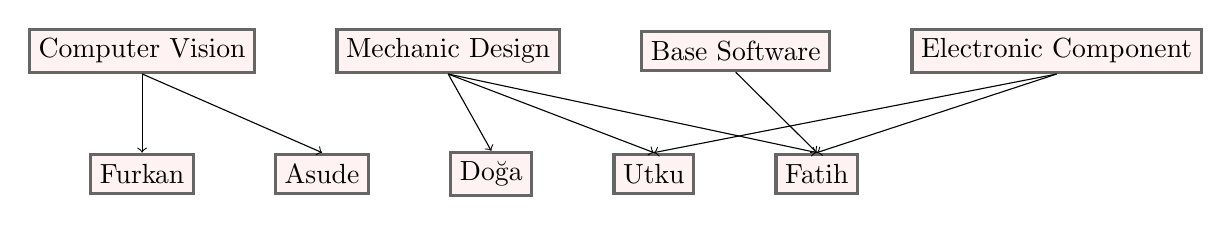
\begin{tikzpicture}[
roundnode/.style={circle, draw=green!60, fill=green!5, very thick, minimum size=7mm},
squarednode/.style={rectangle, draw=black!60, fill=red!5, very thick, minimum size=5mm},
]
% Nodes here..
\node[squarednode] (vis) {Computer Vision};
\node[squarednode] (mec) [right=of vis] {Mechanic Design};
\node[squarednode] (soft) [right=of mec] {Base Software};
\node[squarednode] (ele) [right=of soft] {Electronic Component};
\node[squarednode] (furkan) [below=of vis] {Furkan};
\node[squarednode] (asude) [right=of furkan] {Asude};
\node[squarednode] (doga) [right=of asude] {Doğa};
\node[squarednode] (utku) [right=of doga] {Utku};
\node[squarednode] (fatih) [right=of utku] {Fatih};

% Draw lines..
\draw[->] (mec.south) -- (fatih.north);
\draw[->] (mec.south) -- (utku.north);
\draw[->] (mec.south) -- (doga.north);

\draw[->] (vis.south) -- (furkan.north);
\draw[->] (vis.south) -- (asude.north);

\draw[->] (ele.south) -- (fatih.north);
\draw[->] (ele.south) -- (utku.north);

\draw[->] (soft.south) -- (fatih.north);

\end{tikzpicture}
% TODO - grafik genisletilecek

\section{Team Organization} \label{sec:team_org}

\begin{figure}[htp]
  \centering
  
  
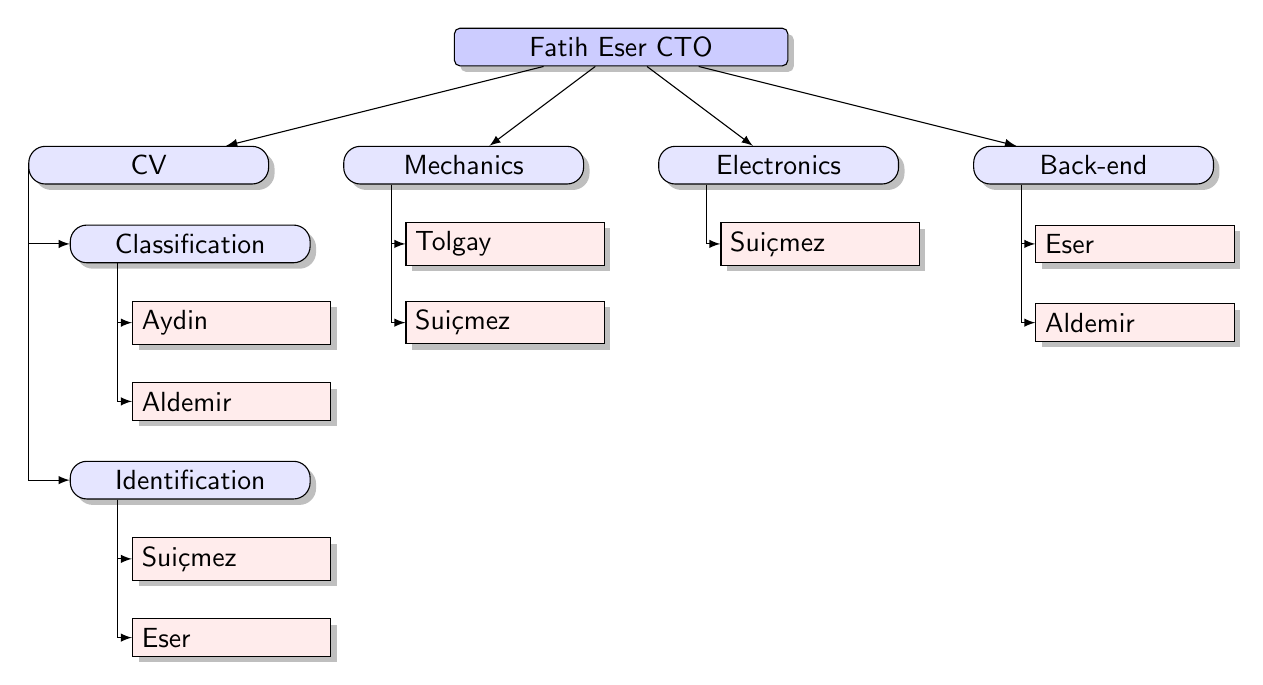
\begin{tikzpicture}[
  level 1/.style={sibling distance=40mm},
  edge from parent/.style={->,draw},
  >=latex,
]

% root...
\node[root] (rootNode) {Fatih Eser CTO}
% Teams...
%   \node[squarenode] (cvTeam) [left=of eeTeam] {Computer Vision Team};
%   \node[squarenode] (eeTeam) [below=of rootNode] {Electronics Team};
%   \node[squarenode] (mechTeam) [ {Mechanics Team};
%   \node[squarenode] (softTeam) {Software Team};

% Teams...
child {node [level 2] (cvTeam) {CV}}
child {node [level 2] (mechTeam) {Mechanics}}
child {node [level 2] (elecTeam) {Electronics}}
child {node [level 2] (softTeam) {Back-end}};



% child {node[level 2, scale=0.7] (classTeam) {Classification}}
% child {node[level 2] (identTeam) {Identification}}

% Workers...
\begin{scope}[every node/.style={level 3}]

% Team classification
\begin{scope}[every node/.style={level 2}]
\node [below of = cvTeam, xshift=15pt] (classTeam) {Classification};
\end{scope}
\node [below of = classTeam, xshift=15pt] (asudeClassTeam) {Aydin}; 
\node [below of = asudeClassTeam] (furkanClassTeam) {Aldemir}; 

% Team identification...
\begin{scope}[every node/.style={level 2}]
\node [below of = furkanClassTeam, xshift=-15pt] (identTeam) {Identification};
\end{scope}
\node [below of = identTeam, xshift=15pt] (serhanIdentTeam) {Suiçmez};
\node [below of = serhanIdentTeam] (eserIdentTeam) {Eser};

\node [below of = mechTeam, xshift=15pt] (tolgayMechTeam) {Tolgay};
\node [below of = tolgayMechTeam] (serhanMechTeam) {Suiçmez};

\node [below of = elecTeam, xshift=15pt] (serhanElecTeam)  {Suiçmez};

\node [below of = softTeam, xshift=15pt] (eserSoftTeam) {Eser};
\node [below of = eserSoftTeam] (furkanSoftTeam) {Aldemir};
\end{scope}

% Sub-team lines...
\draw[->] (cvTeam.west) |- (classTeam.west);
\draw[->] (cvTeam.west) |- (identTeam.west);

% Worker lines...
\draw[->] (classTeam.195) |- (asudeClassTeam.west);
\draw[->] (classTeam.195) |- (furkanClassTeam.west);

\draw[->] (identTeam.195) |- (serhanIdentTeam.west);
\draw[->] (identTeam.195) |- (eserIdentTeam.west);

\draw[->] (mechTeam.195) |- (tolgayMechTeam.west);
\draw[->] (mechTeam.195) |- (serhanMechTeam.west);

\draw[->] (elecTeam.195) |- (serhanElecTeam.west);

\draw[->] (softTeam.195) |- (eserSoftTeam.west);
\draw[->] (softTeam.195) |- (furkanSoftTeam.west);
  
\end{tikzpicture}

\caption{Organizational team structure}
\label{fig:organizational_structure}
\end{figure}

The members of the team have diverse backgrounds and interests; this helps come up with a clear distribution of tasks. Foci of areas differ as follows: control and signal processing for Furkan, control for Asude, Electronics and Biomedical for Utku, Electronics and a double major in physics for Doga. Doga is also a part of the Center for Solar Energy Research and Applications (GUNAM), similary Asude is in an electronics research group (ULTRAMEMS). Therefore in distributing assignments these focused areas have been taken into consideration. 

The head of the company, Fatih Eser, has experiences in Business Management, Computer Engineering and the sub area of Electrical Engineering - Power Systems. Therefore, he has been chosen as a Chief Technology Officer (CTO) due to his clearer understanding of the modules in the project and general background knowledge in project management. 

As given figure \ref{fig:organizational_structure}, Doga has been given the responsibility to accomplish the mechanics of the projects, construction of the cat food container, lid designing, layout of the whole mechanics of the system and durability tests. 

Utku will be held accountable of the electronics part of the project, he will be designing the ultrasonic dog repeller, battery life and its safety, motor of the lid system, sensors such as sonar (for detecting empty volume to estimate remaining cat food) and any extra sensors which might be added later on. 

Asude and Furkan will work on computer vision problems like classification, time dependent testing, preprocessing to filter out noise and outliers, recognition via feature descriptors and any related problems that will be encountered later on. Furkan's internship experience in deep learning will prove useful in the given tasks in this module of the project. 

Fatih is assigned to the software part because of his personal interests and experience in app and website developing. He will be the back-end developer and will be accountable of data transfer, program optimization, interface coding and eventually developing a web based application. 





\section{Requirement Analysis} \label{sec:req_anal}

% iyisiiin 
% :DD
% 

Objectives of the project are feeding only cats, identifying new cats and recognizing them later, deterring dogs from the area, being rechargeable and portable. Also, feeding regime of identified cats are logged by the system.
The status of the food supply and battery, profiles of the cats and feeding logs will be observed in a mobile application.

Requirements of the project:
\begin{itemize}
\item The rechargeable battery is non-removable. The lithium-ion batteries are placed on battery compartment that has power input. The battery will be completely charged in 3 hours.
\item Battery lasts at least five hours. The equipment will run on 18650 Lithium-ion batteries.
\item No attachments to the animals. The animals will be identified in 4 seconds and their feeds will be automatically delivered. 
\item System should be lightweight in order to be carried by a single person. The system will be around 7 kilograms when the reservoir is full. %burdan öncekiler projede verilen requirementlar, alttakiler objective olabilir.
\item To avoid food waste, three or five times of meal will be given to a single cat in a day.
\item The dogs will be deterred with high frequency sounds in order not to damage them. The frequency will be around 30 kHz. However, high frequency sounds also affect cats. We are working for better solutions.
\item Capacity of the reservoir will be 4 kilograms which is around 45 meals.
\item Power usage should be minimized. Low current driven motor will be used.
\item Light bulb will be used at nights. When the motion sensor is activated the bulb will turn on and it will turn off in 2 minutes. By this way, redundant use of electricity will be eliminated.
\item The identification process should be fast. It will last 4 seconds, after cat enters the area. % 3.maddeye benzer oldu
\end{itemize}
\section{Solution Procedure} \label{sec:sol_proc}

% TODO: TAM OLARAK YAPILMASI GEREKENLERİ YAZMADIM AMA ÇOĞUNU YAZDIM. YAZILMASI GEREKEN ŞEYLER: 
% 1: DURATİON YAZILMALI.
% 2: SEQUENCE GÖSTERİLMELİ. 
% TÜM BUNLARI GANTCHART DA GÖSTEREBİLİRİZ DİYE DÜŞÜNDÜM O YÜZDEN YAZMADIM. 
% 3: COMPUTER VİSİON KISMI YAZILMALI.

The project can be divided into four subgroups in order to solve the problems. These subgroups can be seen at team organization part. Different approaches can be applied in order to meet the specifications. As Felerest, our goal is to determine the best solution in order to solve the problems which will be mentioned in this section. 

There exist several problems such as:

1. Determining the cats and dogs from other animals.

2. Categorizing the cats and determining their behaviours. 

3. Giving the right amount of food and water.

4. The amount of food and water left should be shown.

5. Non stop working for 5 hours.

6. Controlling the electronic devices in order to protect the device from over voltage and heat. 

As mentioned in the above section our system should detect and differ cats from dogs. Moreover cats must be categorized and must be given the sufficient amount of food, not more not less. Dogs must escape from the area. In order to honor the specifications, after a lot of research and hard work, innovator designs and effective solutions will be planned.

Mechanical part should be designed, such that system should adjust the necessary amount of food. This can be done by controlling the flow of the food via door. This door must cut the food flow by the command coming from the controller. Therefore it must be a hard solid material that can move easily or rotate by a simple low power motor like a cheap servo\cite{cite:cheapservo}. Low power motor is important since it is cheaper and consumes less energy which is important for satisfying the \(5^{th}\) condition. After deciding the gate type, food mechanism should be integrated to the gate. These two parts should be perfectly matched since controlling the flow of the food is critical for this project. In every sub-step of this mechanical part, tests will be done with a thinking about every detail. Real time examples will be tested on every sub-step.  

Electronics part should be designed such that it must consume low power and should be effective to make critical jobs. This part consists of four different task like: Dog deterring system, design of power electronics, sensor and microprocessor selection and integration, battery selection and placement. Every sub-part is critical since they all contribute to the other parts of the project. The system should deter the dogs without give any harm. This problem can be solved by disturbing the dogs by using a high frequency signal \cite{cite:Dogrepellingdetterent} or using a harmless sprey \cite{cite:Dogrepellingsprey}  that dogs are sensitive. For both of the solutions a controller should be designed such that when there is a threat, the deterring system should be trigger. Since our electronic devices will only work at certain voltage levels, regulators will be needed. After the selection of the electronic devices right regulators will be selected and will be checked if the system runs as expected.  The amount of food and water should be checked by a sensor like sonar or weight sensor. This sensor should be selected such that it should work with a good precision since our controller will depend on that. In order to select the right sensor a web research will be conducted and after selecting the sensor, the necessary test will be done on it until requirements are fulfilled.
Moreover since our design will work for five hours, a battery must be selected according to the power consumption of the circuit. By simulating the power consumption, effective battery will be selected.

Back-end part is responsible for the software part of the project. There will be several problems after and before the detecting animals like transferring video data, communication between microprocessors and server. Moreover in order to be a user friendly, Felerest will develop a website which, user can check the critical informations like voltage and food level. All of this parts requires a good computer knowledge which our team is very capable of doing that. Firstly a good literature search will be done in order to gain the vision to solve these problem. After that, application of this ideas to our project will be done. Testing these solutions with a real world examples, we will conclude also this part.

Computer vision part is responsible for detecting the cats and classify them. In addition to that dogs must be detected as a threat. Since all animals have their characteristic shapes depending on their species, one can use this animal specific details in order to categorize and differ animals. There exist several open source codes which can be used freely. By looking for these codes and improving the necessary parts, detecting our little friends will no longer be a problem.

The planned schedule can be seen below as a Gantt Chart.
 
\subsection{Mechanical Design} \label{sec:sol_proc} % instead of '5.1', just 'a'
\begin{itemize}
\item Immediate response from controller. 

\item Controlling the food flow effectively.

\item Integration of food mechanism.

\item Making realistic tests.

\item Consumption of less power. 
\end{itemize}

\subsection{Electronics Design} \label{sec:sol_proc} % instead of '5.1', just 'a'

\begin{itemize}
\item Deterring the dogs without giving any harm. 

\item Selecting the right sensor, microprocessor and regulator.

\item Calculating the overall power of the system and selecting the right battery. 

\item Generating a good control mechanism for the overheating and overvoltage.

\item Making real time tests.

\end{itemize}

\subsection{Computer Vision} \label{sec:sol_proc} % instead of '5.1', just 'a'
\begin{itemize}
\item Making a search for features of the cats and dogs.

\item Searching for open source codes. 

\item Improving and implementing codes. 

\item Testing and concluding the CV part.  

\end{itemize}
\subsection{Back-end software Framework} \label{sec:sol_proc} % instead of '5.1', just 'a'
\begin{itemize}
\item Transferring video data. 

\item Establishing the communication between microprocessors and server.

\item Designing the interface for computer camera and website.

\item Building a user friendly website.

\item Testing and concluding.
\end{itemize}
%Computer vision part is responsible for detecting the cats and classify them. In addition to that dogs must be detected as a thread. Since all animals have their characteristic shapes depending on their species, one can use this animal specific details in order to categorize and differ animals. There exist several open source codes which can be used freely. By looking for these codes and improving the necessary parts, detecting our little friends will no longer be a problem.

%Back-end part is responsible for the software part of the project. There will be several problems after and before the detecting animals like transferring video data, communication between microprocessors and server. Moreover in order to be a user friendly, Felerest will develop a website which, user can check the critical informations like voltage and food level. All of this parts requires a good computer knowledge which our team is very capable of doing that. Firstly a good literature search will be done in order to gain the vision to solve these problem. After that, application of this ideas to our project will be done. Testing these solutions with a real world examples, we will conculude also this part.


\section{Deliverables} \label{sec:deliverables}
\begin{itemize}
\item The box that only feed the cats.

\item The sensors which will show the food and water level. 

\item The sensors which will show the battery level. 

\item Mobile application that will show food, water and battery level. Moreover this application will show the feeding regimes of the different cats. 

\item Feeding diets of the various cats.

\item Business Statement Report 

\item Proposal Report

\item Conceptual Design Report
\end{itemize}
\section{Conclusion}
\label{sec:conclusion}




\bibliographystyle{plain}
\bibliography{ref}

\end{document}




% TODO - team organization chartı yapılacak, time dependence arastırılıp gantt charta konulacak weekly report yazılacak

% TODO - kisaltmalari aciklayacagiz